\section{Introduction}
\label{s:secIntroLHC}
The European Organisation for Nuclear Research 
(CERN- \emph{Conseil Europ\'{e}n pour la Recherche Nucl\'{e}aire}), located at Geneva, 
Switzerland, is one of the leading laboratories in the world in the field of experimental 
high energy physics. The experimental collaborations at CERN involve more than 1700 people 
from 41 countries. The research activity at CERN ranges from the understanding of fundamental 
constituents of matter such as the Higgs Boson to the hunt of dark matter. Particles such as protons 
(p), lead nuclei (Pb) are accelerated to a very high speed (nearly the speed of light) and collided 
head-on. The acceleration of these particles proceeds in several stages, such as shown in Figure 
\ref{fig:lhc}.
\begin{figure}
  \begin{center}
  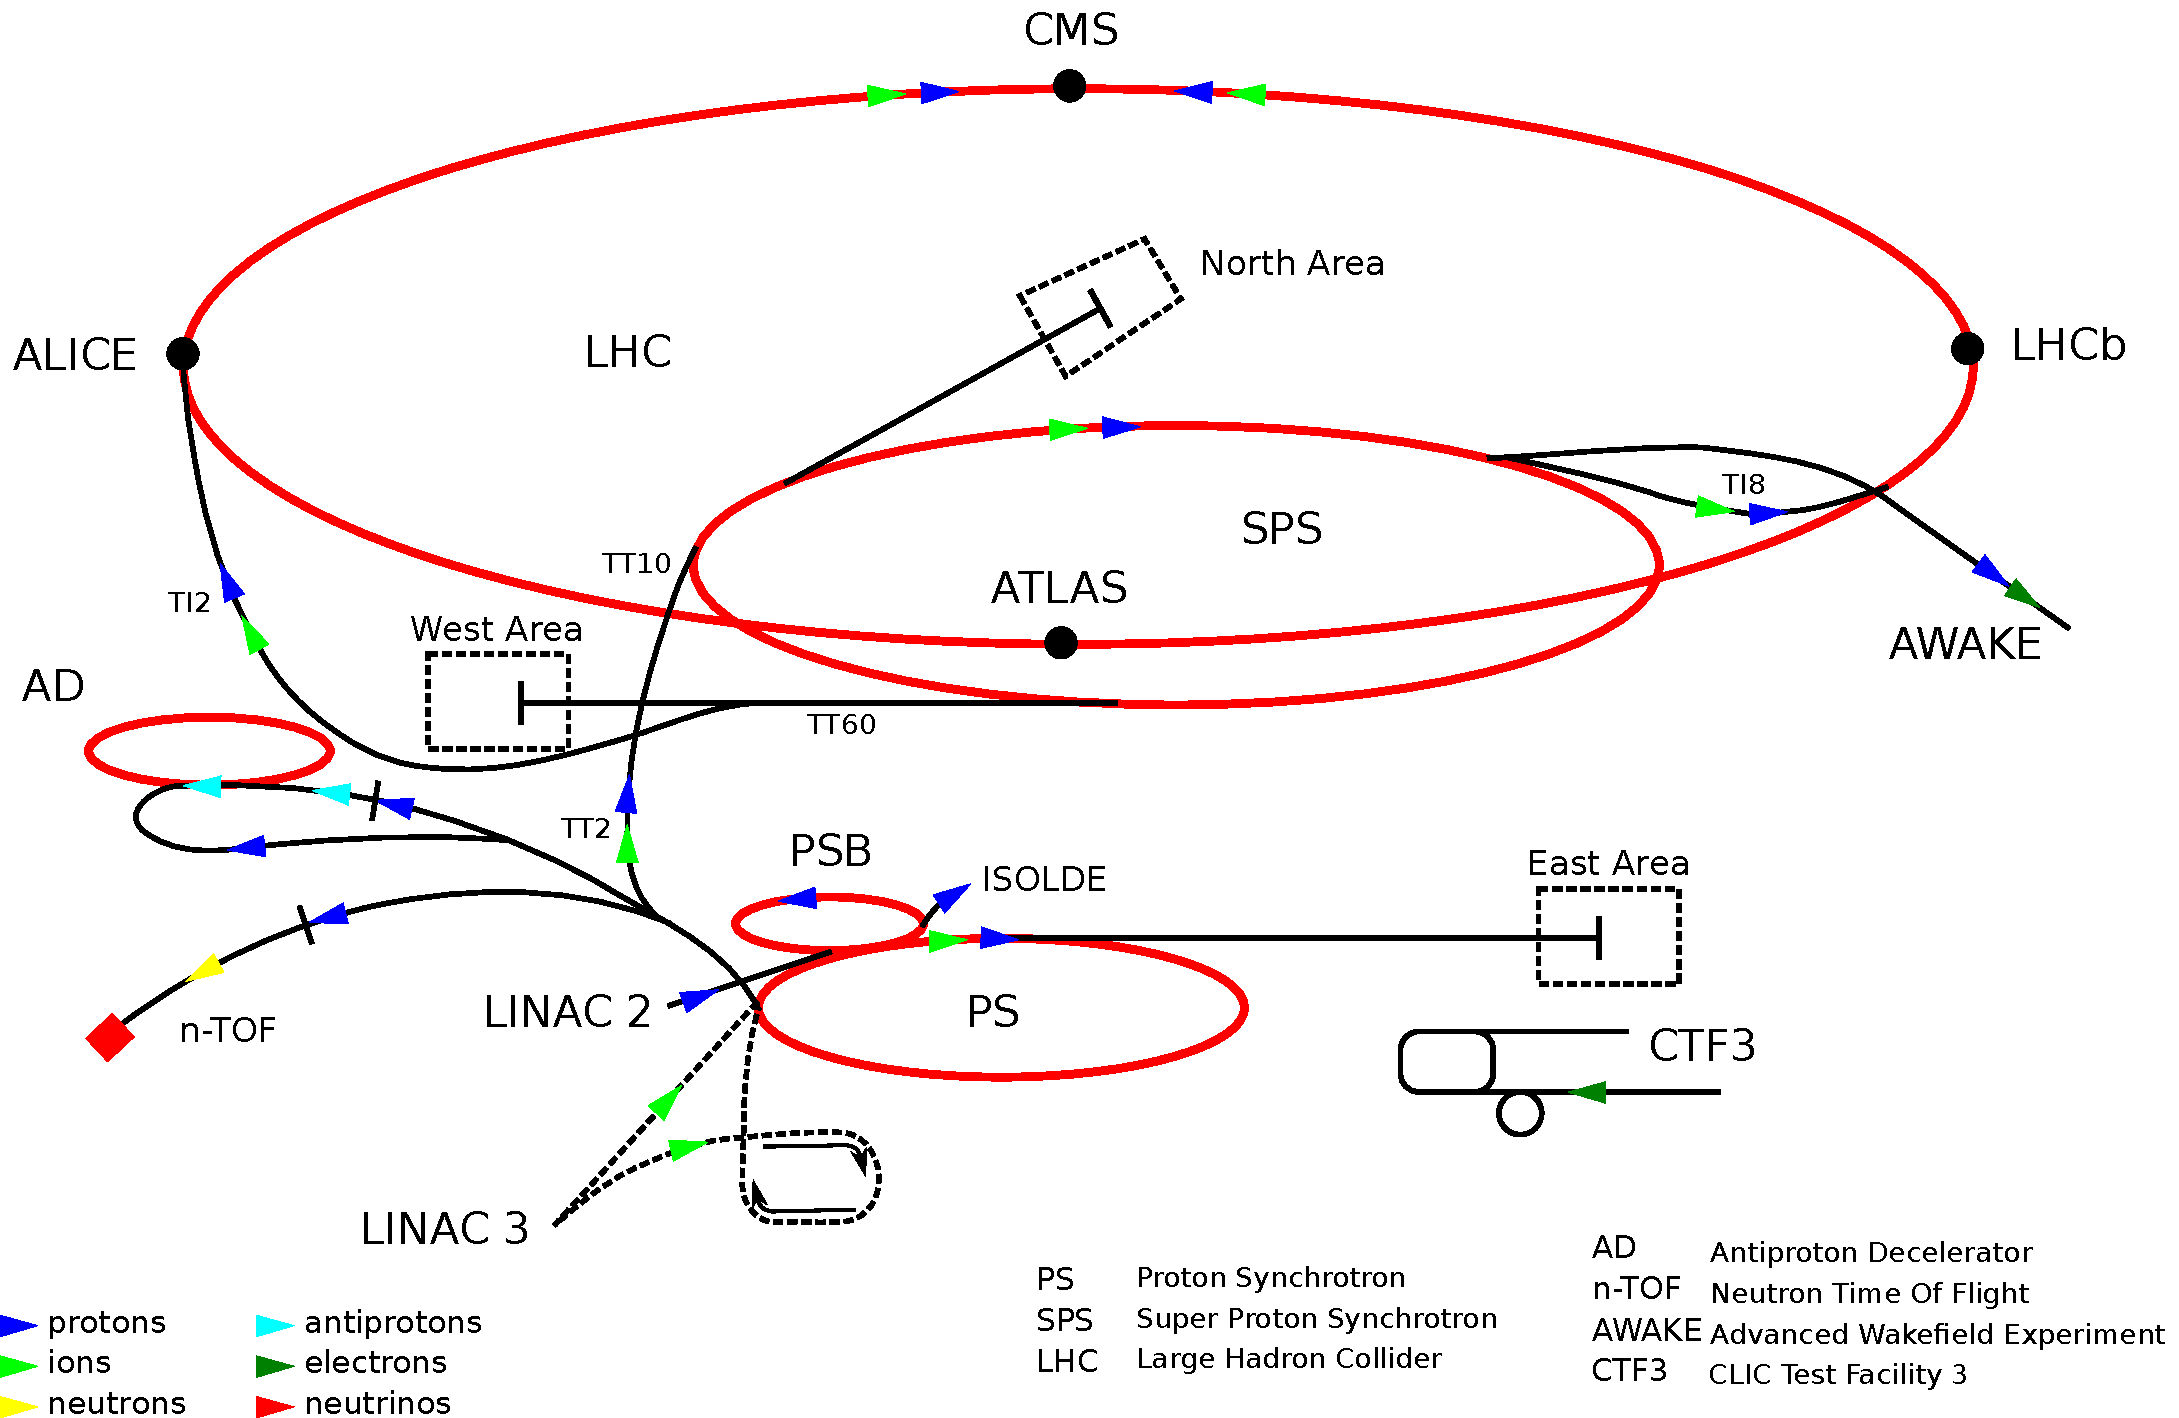
\includegraphics[width=0.80\linewidth]{Experiment/LHC/Image/cernacc.pdf}
  \caption{The CERN accelerator complex~\cite{wiki:cernAcc}. The particles are accelerated 
	at various stages, starting from LINAC to PSB to PS to SPS to LHC. Various detectors 
	such as ATLAS, LHCb, CMS, and ALICE are placed at the collision points.}
  \label{fig:lhc}
  \end{center}
\end{figure}

Bunches of protons (\emph{$H^+$}, after the electron is stripped-off from a hydrogen 
atom) are first passed through the Linear Accelerator (LINAC2), which accelerates the 
protons to an energy of 50 \MeV. Subsequently, the proton bunches are passed through the 
Proton Synchrotron Booster (PSB) which accelerates the protons to an energy of 1.4 \GeV.
Further, the bunches are circulated in a bigger Proton Synchrotron (PS) accelerating protons 
up to an energy of 26 \GeV. After that, the proton bunches are circulated 
inside the Super Proton Synchrotron (SPS) which accelerates them to an energy of 
450 \GeV. Finally, the bunches are injected into the Large Hadron Collider (LHC)
ring. Where protons are accelerated to a speed of 99.99\% of the speed of light.
At such a large speed the proton bunches come so close that they look like a beam. 
The increment in the energy of protons at various stages are listed in 
Table~\ref{tab:lhc}.
\begin{table} 
\caption{\label{tab:lhc} The energy of protons after passing through various 
	accelerators.} 
\begin{centering} 
\begin{tabular}{cc} 
\hline  
\hline 
\noalign{\vskip 0.1cm}
LINAC2 & 50 \MeV \tabularnewline 
\noalign{\vskip 0.1cm}
PSB & 1.4 \GeV \tabularnewline 
\noalign{\vskip 0.1cm}
PS & 26 \GeV \tabularnewline 
\noalign{\vskip 0.1cm}
SPS & 450 \GeV \tabularnewline 
\noalign{\vskip 0.1cm}
LHC & 7 \TeV \tabularnewline 
\hline  
\hline 
\end{tabular} 
\par\end{centering} 
\end{table}

A typical synchrotron consists of many components such as dipole magnets to bend the beams,
quadrupole magnets to focus the beams, radio frequency (RF) cavities to accelerate
the beams, cryogenics for superconducting and cooling the LHC ring, and beam diagnostics
to monitor the beam movement.
Two proton beams, moving in the opposite direction, are collided at four points of 
the LHC ring, as shown in Figure~\ref{fig:lhcRing}. 
\begin{figure}
  \begin{center}
  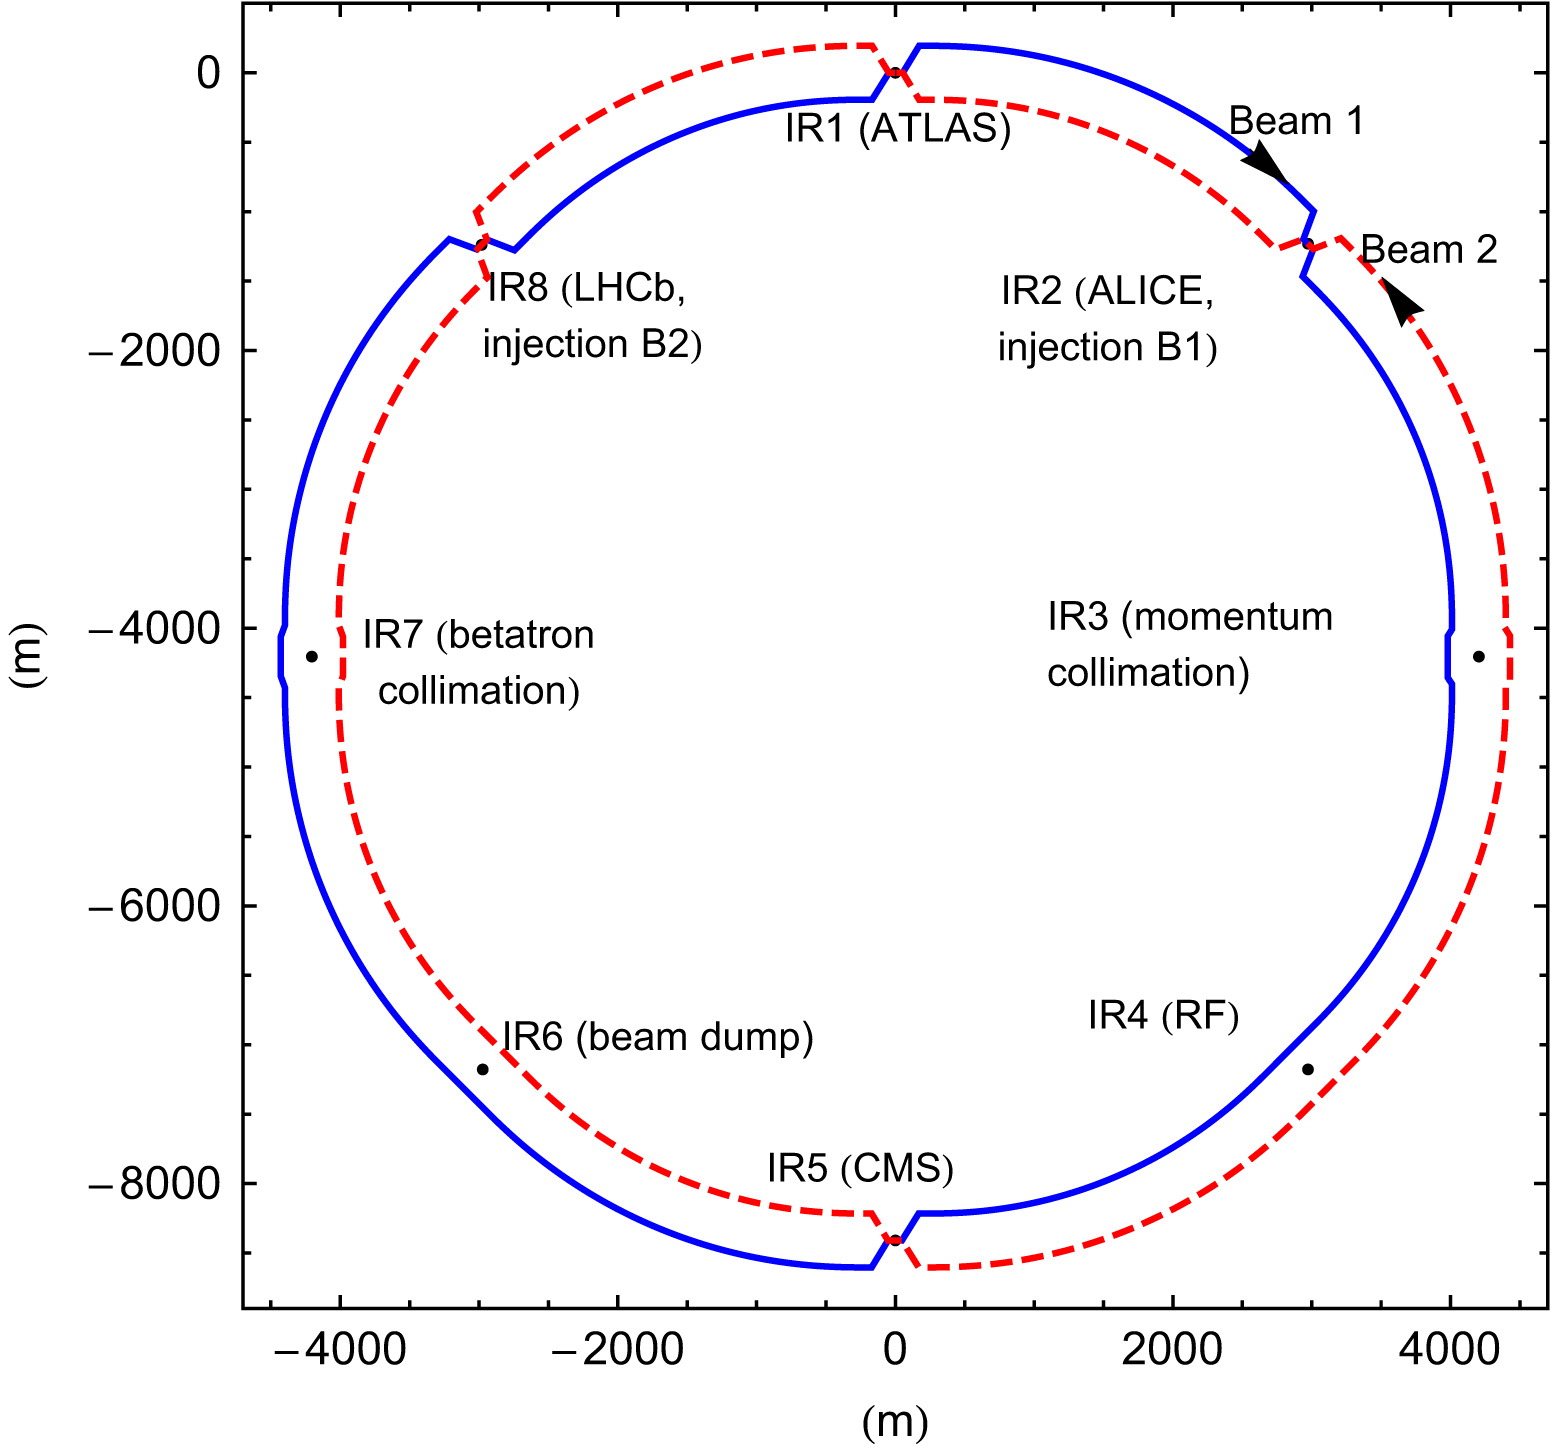
\includegraphics[width=0.50\linewidth]{Experiment/LHC/Image/lhc_ring.jpg}
	  \caption{The layout of insertion regions (IRs) at the LHC ring \cite{BRUCE2013825}.
	  The separation between the two colliding beams is not to scale. The 
	  separation between them is exaggerated for illustration. The total circumference
	  of the LHC ring is 27\unit{km}. Oppositely moving beams (Beam 1 and 2) are made 
	  to collide at four points of the ring. At the collision points, detectors such as
	  CMS, ALICE, ATLAS, and LHCb are installed to record the collision.}
  \label{fig:lhcRing}
  \end{center}
\end{figure}

There are eight insertion regions (IRs) at the LHC ring as shown in Figure~\ref{fig:lhcRing}. 
At four of them, where collision happens, four main detectors are installed,
ATLAS at IR1, ALICE at IR2, CMS at IR5, and LHCb at IR8. Three other small detectors namely 
LHCf, TOTEM, and MoEDAL are placed in the same cavern as ATLAS, CMS, and LHCb, 
respectively. At other IRs, the collimators are installed 
such as the momentum collimator at IR3, betatron at IR7, and RF at IR4. The beam dumping system 
is placed at IR6. Near the collision points, various systems such as dipole and quadrupole
magnets are installed to bend and focus the proton beams as shown in Figure~\ref{fig:lhc_beamBend}.
Using these magnets the two counter rotating beams are brought closer for a head-on
collision. A brief description of various detectors is given in the next section.
%https://cds.cern.ch/record/2207171/plots
\begin{figure}
  \begin{center}
  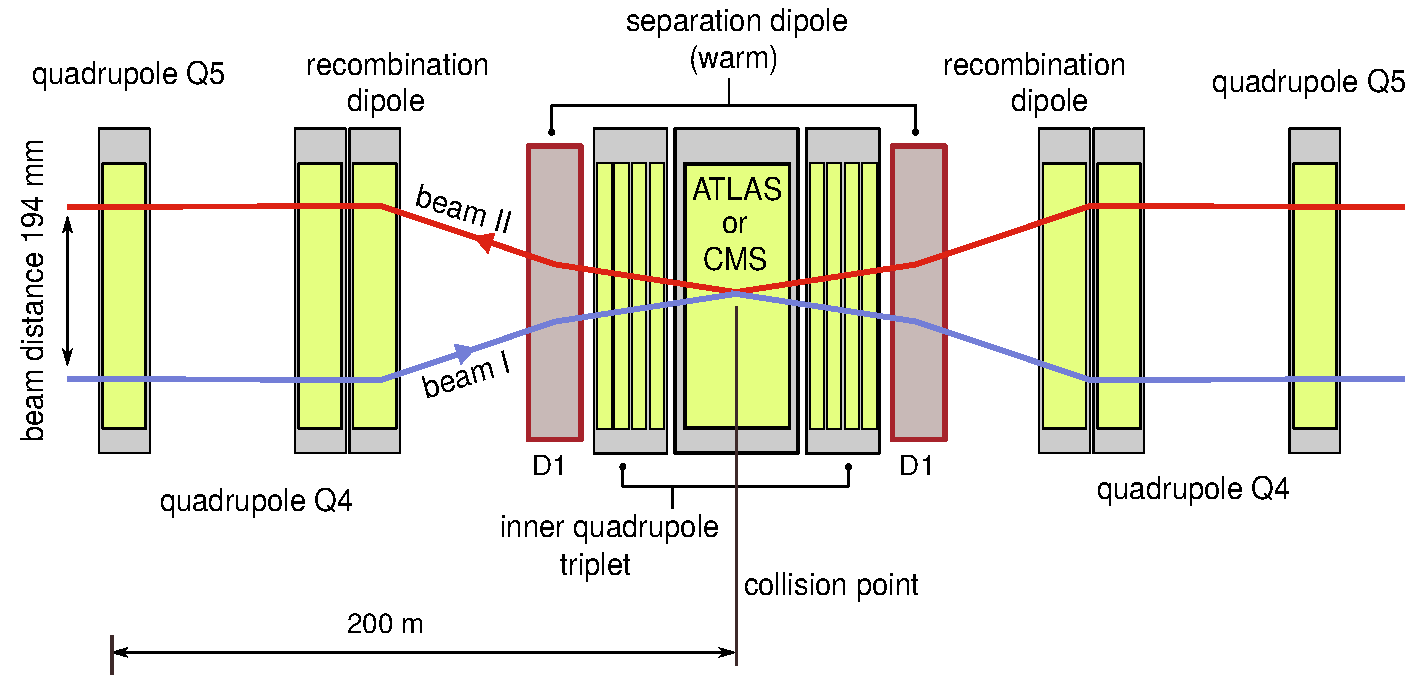
\includegraphics[width=0.75\linewidth]{Experiment/LHC/Image/lhc_beamBend.pdf}
  \caption{Schematic diagram showing quadrupole and dipole magnets 
	  for focussing and bending proton beams at the interaction point (IP). 
	The D1 dipole separate beams from both sides of the IP. This figure is adopted 
	from \cite{Schmidt:2207171}.}
  \label{fig:lhc_beamBend}
  \end{center}
\end{figure}
